\renewcommand{\theequation}{\theenumi}
\begin{enumerate}[label=\thesubsection.\arabic*.,ref=\thesubsection.\theenumi]
\numberwithin{equation}{enumi}

\item $p\brak{x, y} = Ax^2 + Bxy + Cy^2 + Dx + Ey + F$ can be represented as follow in the vector form:
\begin{align}
\vec{x}^T 
\myvec{
A & \frac{B}{2} \\
\frac{B}{2} & C
}
\vec{x} + 
\myvec{
D & E 
}
\vec{x} + F = 0
\end{align}

\item To solve the equation - $3x^2-4x+\frac{20}{3} = 0$: 
\begin{flushleft}
The given equation can be represented as follows in the vector form:
\end{flushleft}
\begin{align}
\vec{x}^T 
\myvec{
3 & 0 \\
0 & 0
}
\vec{x} + 
\myvec{
-4 & 0 
}
\vec{x} + \frac{20}{3} = 0 \label{eq:conics_main}
\end{align}

\item To find the roots $y=0$:
\begin{align}
\vec{x} = \myvec{x\\0} \\
3x^2-4x+\frac{20}{3} &= 0 \\
\brak{x-\myvec{\frac{2}{3}\\ \frac{2\sqrt{14}}{3}}}\brak{x-\myvec{\frac{2}{3}\\\frac{-2\sqrt{14}}{3}}} &= 0 \\
x = \myvec{\frac{2}{3}\\ \frac{2\sqrt{14}}{3}},\myvec{\frac{2}{3}\\ \frac{-2\sqrt{14}}{3}}
\end{align}

\item To verify:\\
Figure \ref{fig:quadeq1_conics_ex} show that the equation does not intersect the x-axis hence there are no real roots. 

\begin{figure}[!ht]
\centering
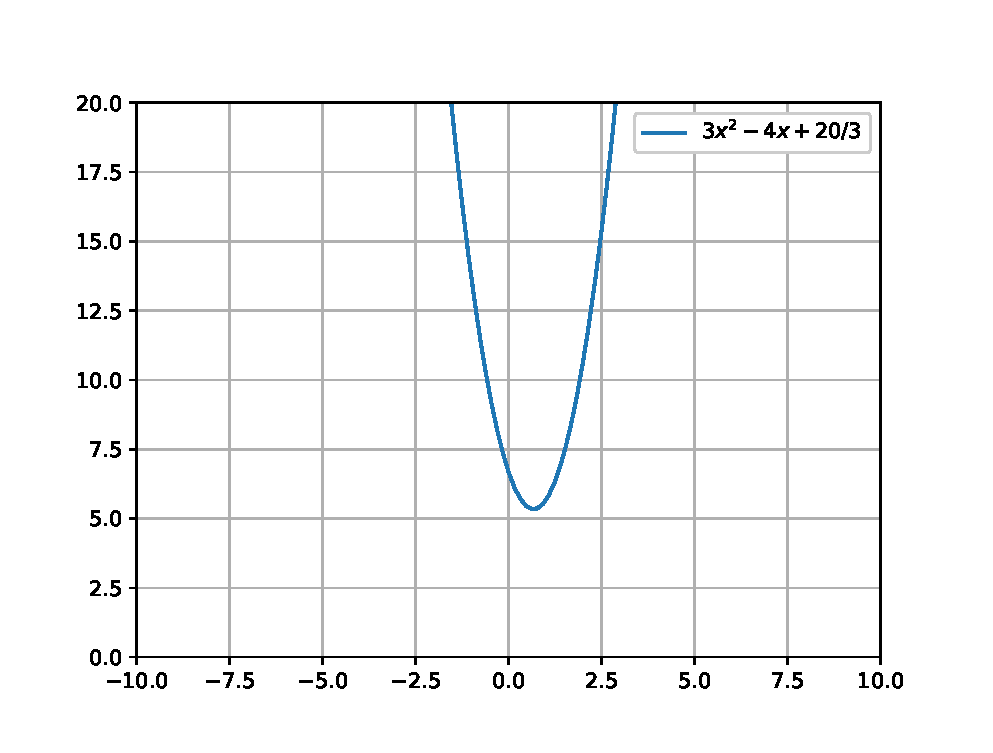
\includegraphics[width=\columnwidth]{./figs/conics_ex/quadratic_equation_1.eps}
\caption{$3x^2-4x+\frac{20}{3}$ generated using python}
\label{fig:quadeq1_conics_ex}
\end{figure} 
%%%%%%%%%%%%%%%%%%%%%%
\item To solve the equation - $x^2-2x+\frac{3}{2} = 0$: 
\begin{flushleft}
The given equation can be represented as follows in the vector form:
\end{flushleft}
\begin{align}
\vec{x}^T 
\myvec{
1 & 0 \\
0 & 0
}
\vec{x} + 
\myvec{
-2 & 0 
}
\vec{x} + \frac{3}{2} = 0 \label{eq:conics_main}
\end{align}

\item To find the roots $y=0$:
\begin{align}
\vec{x} = \myvec{x\\0}\\
x^2-2x+\frac{3}{2} &= 0 \\
\brak{x-\myvec{1 \\ \sqrt{2}}}\brak{x - \myvec{1\\ -\sqrt{2}}} &= 0 \\
x = \myvec{1\\ \sqrt{2}}, \myvec{1\\ -\sqrt{2}}
\end{align}

\item To verify:\\
Figure \ref{fig:quadeq2_conics_ex} show that the equation does not intersect the x-axis hence there are no real roots.

\begin{figure}[!ht]
\centering
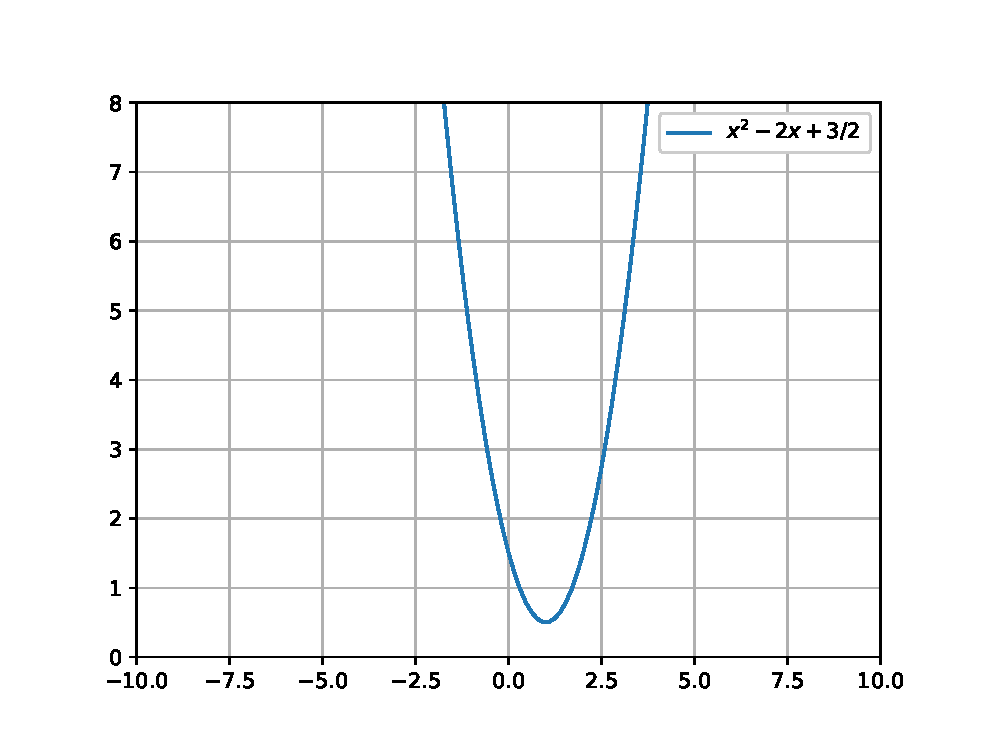
\includegraphics[width=\columnwidth]{./figs/conics_ex/quadratic_equation_2.eps}
\caption{$x^2-2x+\frac{3}{2}$ generated using python}
\label{fig:quadeq2_conics_ex}
\end{figure} 
%%%%%%%%%%%%%%%%%%%%%%
\item To solve the equation - $27x^2-10x+1 = 0$: 
\begin{flushleft}
The given equation can be represented as follows in the vector form:
\end{flushleft}
\begin{align}
\vec{x}^T 
\myvec{
27 & 0 \\
0 & 0
}
\vec{x} + 
\myvec{
-10 & 0 
}
\vec{x} + 1 = 0 \label{eq:conics_main}
\end{align}

\item To find the roots $y=0$:
\begin{align}
\vec{x} = \myvec{x\\0} \\
27x^2-10x+1 &= 0 \\
\brak{x-\myvec{\frac{5}{27} \\ \  \frac{\sqrt{2}}{27}}}\brak{x - \myvec{\frac{5}{27} \\ \ \frac{-\sqrt{2}}{27}}} &= 0 \\
x = \myvec{\frac{5}{27} \\ \  \frac{\sqrt{2}}{27}}, \myvec{\frac{5}{27} \\ \  \frac{-\sqrt{2}}{27}}
\end{align}

\item To verify:\\
Figure \ref{fig:quadeq3_conics_ex} show that the equation does not intersect the x-axis hence there are no real roots.

\begin{figure}[!ht]
\centering
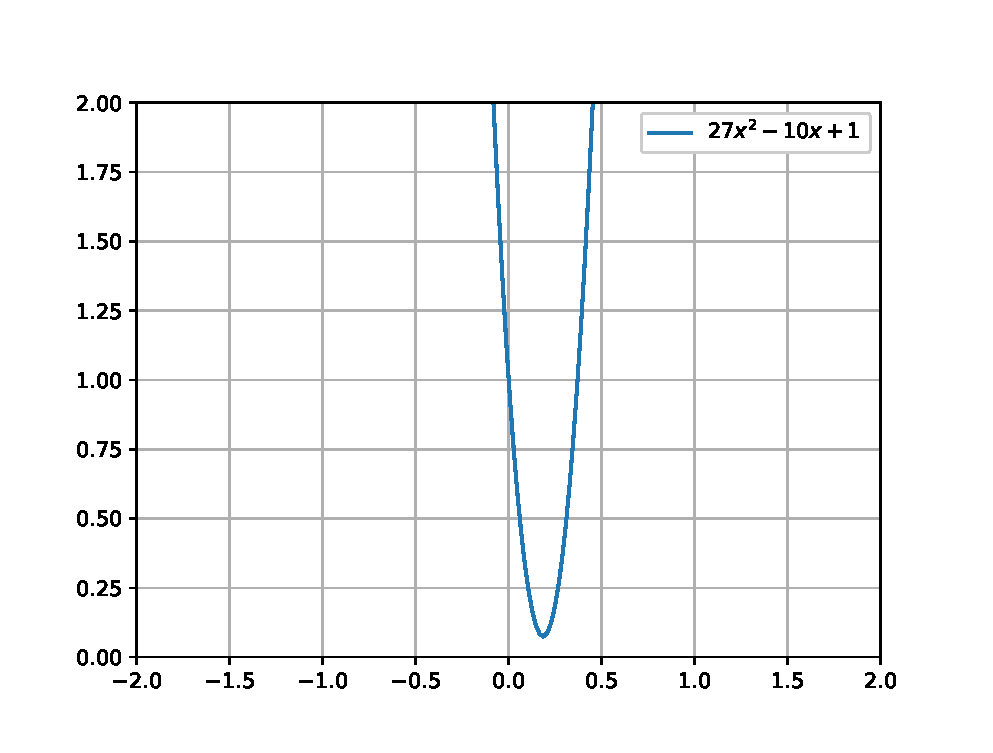
\includegraphics[width=\columnwidth]{./figs/conics_ex/quadratic_equation_3.eps}
\caption{$27x^2-10x+1$ generated using python}
\label{fig:quadeq3_conics_ex}
\end{figure} 
%%%%%%%%%%%%%%%%%%%%%%
\item To solve the equation - $21x^2-28x+10 = 0$: 
\begin{flushleft}
The given equation can be represented as follows in the vector form:
\end{flushleft}
\begin{align}
\vec{x}^T 
\myvec{
21 & 0 \\
0 & 0
}
\vec{x} + 
\myvec{
-28 & 0 
}
\vec{x} + 10 = 0 \label{eq:conics_main}
\end{align}

\item To find the roots $y=0$:
\begin{align}
\vec{x} = \myvec{x\\0}\\
21x^2-28x+10 &= 0 \\
\brak{x-\myvec{\frac{2}{3} \\\  \frac{\sqrt{14}}{21}}}\brak{x - \myvec{\frac{2}{3} \\\  \frac{-\sqrt{14}}{21}}} &= 0 \\
x = \myvec{\frac{2}{3} \\\  \frac{\sqrt{14}}{21}}, \myvec{\frac{2}{3} \\\  \frac{-\sqrt{14}}{21}}
\end{align}

\item To verify:\\
Figure \ref{fig:quadeq4_conics_ex} show that the equation does not intersect the x-axis hence there are no real roots.

\begin{figure}[!ht]
\centering
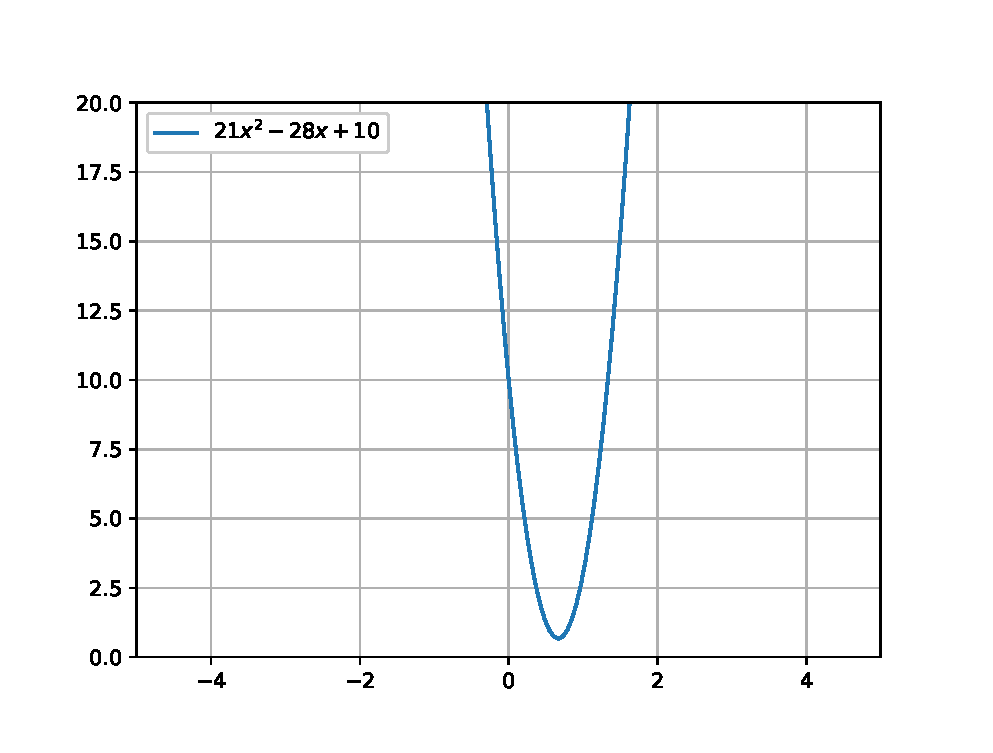
\includegraphics[width=\columnwidth]{./figs/conics_ex/quadratic_equation_4.eps}
\caption{$21x^2-28x+10$ generated using python}
\label{fig:quadeq4_conics_ex}
\end{figure} 
%%%%%%%%%%%%%%%%%%%%%%

The  following Python code generates Fig.\ref{fig:quadeq1_conics_ex}, \ref{fig:quadeq2_conics_ex}, \ref{fig:quadeq3_conics_ex} and \ref{fig:quadeq4_conics_ex} 

\begin{lstlisting}
codes/conics_ex/conics_ex.py
\end{lstlisting}
\end{enumerate}